
\section{Symmetric Cryptography}

\paragraph{One-time pad}
Plaintext $p$, key $k$ such that $|p| = |k|$.
Ciphertext $c = p \xor k$.

If $k$ u.a.r. and only used once then the OTP is \textbf{perfectly secure}, i.e.
$ \Pr[P=p|C=c] = \Pr[P=p]$.

Note: keys can re-occur (as a result of random sampling) but they must not be re-used (i.e. the adversary must not be aware that the same key is used).

Issues: same lengths, key distribution, single use.

\subsection{Block Ciphers}

\paragraph{Block cipher}
A block cipher with key length $k$ and block size $n$ consists of two efficiently computable permutations\footnote{Encipher and decipher}:
$$ E: \setzeroone^k \times \setzeroone^n \mapsto \setzeroone^n \quad
D: \setzeroone^k \times \setzeroone^n \mapsto \setzeroone^n $$
such that for all keys $K$ $D_K$ is the inverse of $E_K$
(where we write $E_K$ short for $E(K, \cdot)$).

\paragraph{Security notions}
Known plaintext attack, chosen plaintext attack, chosen ciphertext attack.
Exhaustive key search on $(P,C)$ pairs -- no attack should be better, else we throw the cipher away.

\paragraph{Pseudo-randomness}
\begin{itemize}
\item Adversary $\A$ interacts either with block cipher $(E_K, D_K)$ or a truly random permutation $(\Pi, \Pi^{-1})$.
\item A block cipher is called a \textbf{pseudo-random permutation PRP} if no efficient\footnote{Quantified by runtime + number of oracle queries.} $\A$ can tell the difference between $E_K$ and $\Pi$ (no access to the inverse).
\item A block cipher is called a \textbf{strong-PRP} if no efficient $\A$ can tell the difference between $(E_K, D_K)$ and $(\Pi, \Pi^{-1})$.
\end{itemize}

\begin{figure}[h]
    \centering
	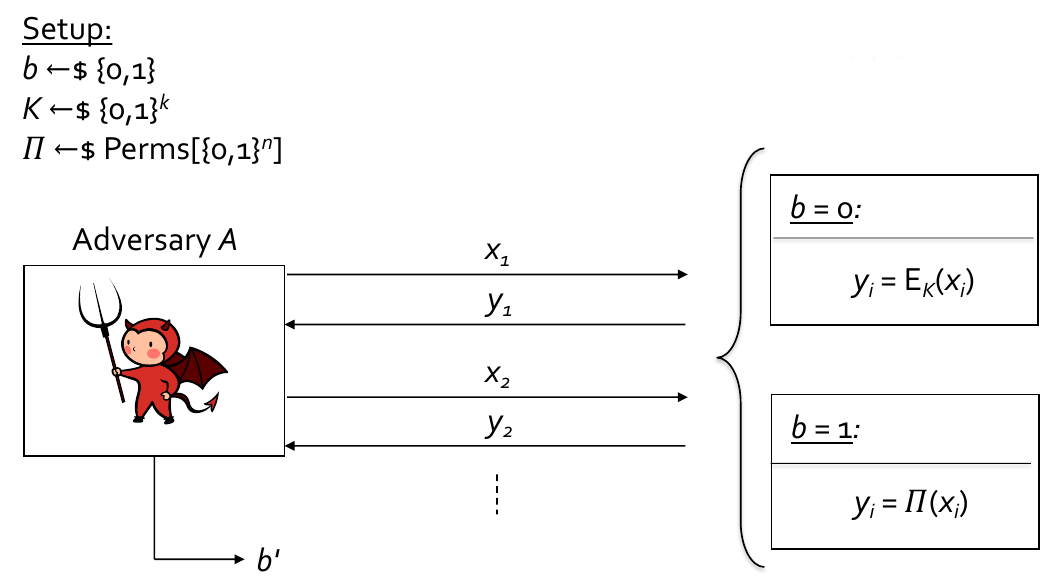
\includegraphics[scale=0.4]{images/prp.png}
    \caption{PRP game}
    \label{fig:prp}
\end{figure}

The advantage is defined as:
$$
\mathbf{Adv}^{PRP}_E (\A)
= 2 \cdot \Big| \Pr[ \text{Game }\textbf{PRP}(\A, E) \Rightarrow \text{true} ] - \frac{1}{2} \Big|
$$
where the probability is over the randomness of $b, K, \Pi, \A$.
Note that:
$$
\Pr[ \text{Game }\textbf{PRP}(\A, E) \Rightarrow \text{true} ]
= \Pr[b'=b]
$$
Also see the Advantage Rewriting Lemma (\ref{adv-rewr-lemm}).

\paragraph{Constructing block ciphers}
In general: keyed round function that is repeated many times.

\begin{itemize}
\item Feistel cipher: halved blocks crossing back and forth, e.g. DES
\item Substitution-permutation network: confusion + diffusion, e.g. AES
\end{itemize}

\paragraph{Electronic Code Book (ECB) mode}
Same plaintext always maps to the same ciphertext (deterministic).
Thus serious leakage, don't use.

\begin{figure}[h]
    \centering
	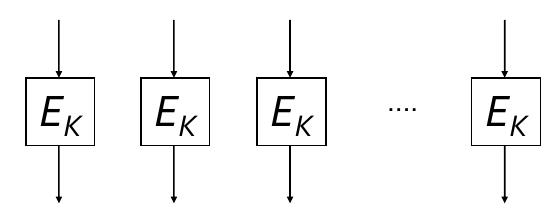
\includegraphics[scale=0.4]{images/ecb.png}
    \caption{ECB mode}
    \label{fig:ecb}
\end{figure}

\paragraph{Cipher Block Chaining (CBC) mode}
Use u.a.r. IV/previous ciphertext block to randomise encryption.

A bit flip in $C_i$ completely scrambles/randomises $P_i$ and flips the same bit in $P_{i+1}$.

Caveats: non-random IV, padding oracle attack, ciphertext block collisions (after using the same key for $2^{n/2}$ blocks by the birthday bound).

\begin{figure}[h]
    \centering
	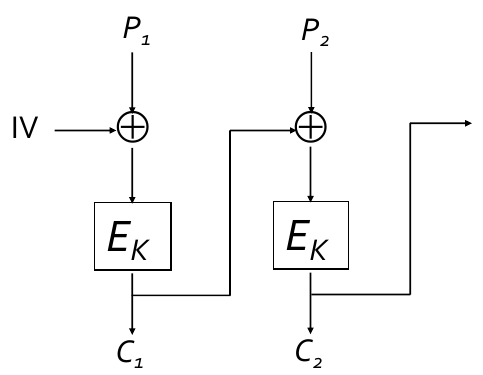
\includegraphics[scale=0.4]{images/cbc-enc.png}
	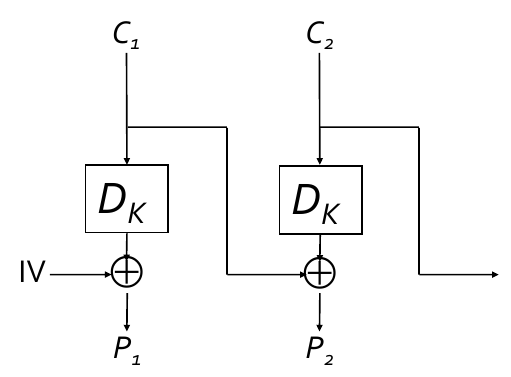
\includegraphics[scale=0.4]{images/cbc-dec.png}
    \caption{CBC mode (left: encipher, right: decipher)}
    \label{fig:cbc}
\end{figure}

\paragraph{Counter (CTR) mode}
Incrementing counter is encrypted with block cipher to produce a pseudo-random value to xor the plaintext block with.

Effectively a stream cipher producing OTP keys.
$E_K$ does not even need to be invertible.
No padding needed, can just truncate the last block.
A bit flip it $C_i$ flips the same bit in $P_i$.

Caveats: counter must not repeat/wrap around (else xor of ciphertexts = xor of plaintexts).

\begin{figure}[h]
    \centering
	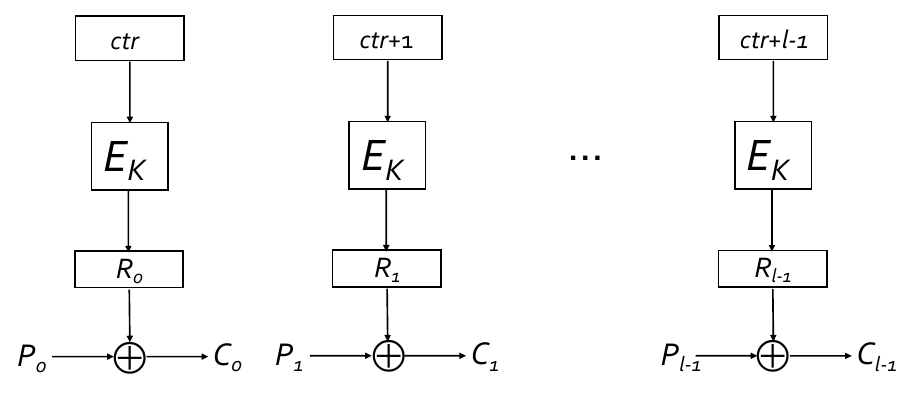
\includegraphics[scale=0.4]{images/ctr.png}
    \caption{CTR mode}
    \label{fig:ctr}
\end{figure}



\subsection{Symmetric Encryption}

\paragraph{Symmetric Encryption Scheme}
is a triple $ SE = (KGen, Enc, Dec) $.
We have key space $\K = \setzeroone^k$, message space $\M = \setzeroone^*$\footnote{In reality we might have a maximum plaintext length.} and ciphertext space $\C = \setzeroone^*$.
For correctness, we have $ Dec_K(Enc_K(m))=m $.

\paragraph{IND-CPA Security}
Informally:
computational version of perfect security --
an efficient adversary cannot compute anything useful from a ciphertext (e.g. hide every bit of the plaintext).
Equivalent to \emph{semantic security}.

Formally:
For any efficient adversary $\A$, given the encryption of one of two equal-length messages of its choice,
$\A$ is unable to distinguish which one of the two messages was encrypted.

In the security game, $\A$ gets access to a \emph{Left-or-Right encryption oracle}.
The advantage of $\A$ is:
$$
\adv^{IND-CPA}_{SE} (\A)
= 2 \cdot \Big| \Pr[ \text{Game }\textbf{IND-CPA}(\A, SE) \Rightarrow \text{true} ] - \frac{1}{2} \Big|
$$

Notes:
Deterministic schemes \textbf{cannot} be IND-CPA secure (why?).
CBC and CTR mode (if used properly) can be proven to be IND-CPA secure (assuming that $Enc$ is a PRP-secure block cipher).

Caveats:
No integrity. Says nothing about messages of non-equal length. No chosen ciphertexts.

\begin{figure}[h]
    \centering
	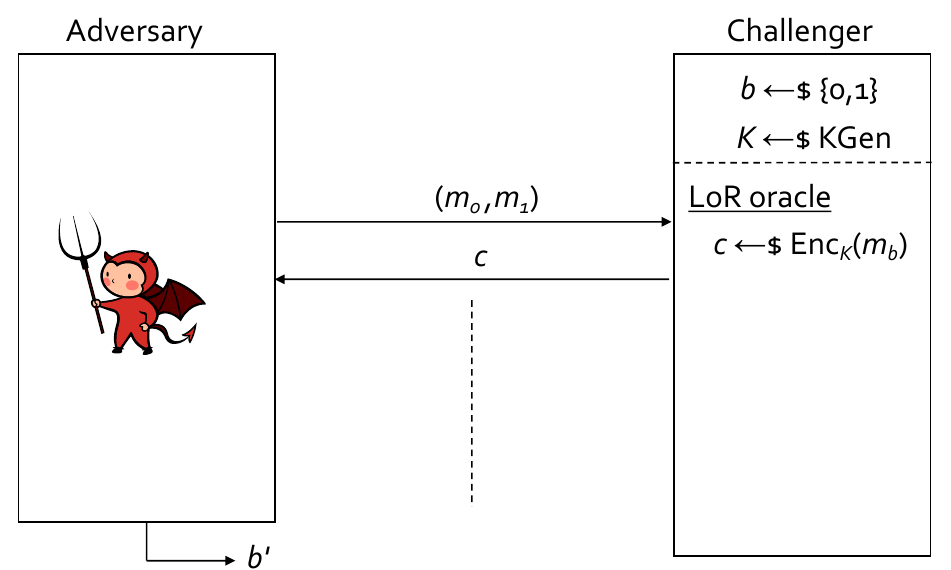
\includegraphics[scale=0.4]{images/ind-cpa.png}
    \caption{IND-CPA game}
    \label{fig:ind-cpa}
\end{figure}

\paragraph{Advantage Rewriting Lemma}\label{adv-rewr-lemm}
Let $b$ be a uniformly random bit and $b'$ the output of some algorithm. Then:
\begin{align*}
2 \Big| \Pr[b'=b] - \frac{1}{2} \Big|
&= \Big| \Pr[b'=1|b=1] - \Pr[b'=1|b=0] \Big| \\
&= \Big| \Pr[b'=0|b=0] - \Pr[b'=0|b=1] \Big|
\end{align*}

\paragraph{Difference Lemma}
Let $Z, W_1, W_2$ be events. If
$$
(W_1 \wedge \neg Z) \text{ occurs if and only if } (W_2 \wedge \neg Z) \text{ occurs}
$$
then
$$
\Big| \Pr[W_2] - \Pr[W_1] \Big| \leq \Pr[Z]
$$
In practice: $Z$ is a bad event that rarely happens, $W_1, W_2$ are when $\A$ wins in security games $G_1, G_2$.
Useful for \emph{game hopping} proofs.

\paragraph{PRP-PRF Switching Lemma}
Let $E$ be a block cipher.
Then for any algorithm $\A$ making $q$ queries:
$$
\Big| \adv^{PRP}_{E} (\A) - \adv^{PRF}_{E} (\A) \Big| \leq \frac{q^2}{2^{n+1}}
$$



\subsection{Attacks}

\paragraph{Padding}
Added before encryption to expand plaintext to a multiple of the block size, i.e. \\$pad(\cdot): \setzeroone^* \mapsto \{ \setzeroone^n \}^*$.
Must be expanding (why?) and efficiently computable.
May be either randomised or deterministic.
\\
E.g. TLS padding: appends $t+1$ bytes of value $t$.

Problem: adversary can detect padding errors (explicit error messages, logs, timing differences).

\paragraph{Padding Oracle}
Given a ciphertext $C$, returns whether the padding of the decryption is valid or invalid.
Leaks 1 bit of information.
Kind of a chosen ciphertext attack, thus \underline{not} covered by IND-CPA security!
Main problem: no ciphertext integrity.

In practice:
$\A$ needs 128 oracle queries on average to recover one plaintext byte.
Repeat for all bytes and all blocks for full plaintext recovery.
Additional practical details to consider.
For TLS attacks, see Lucky 13 and POODLE.

\begin{figure}[h]
    \centering
	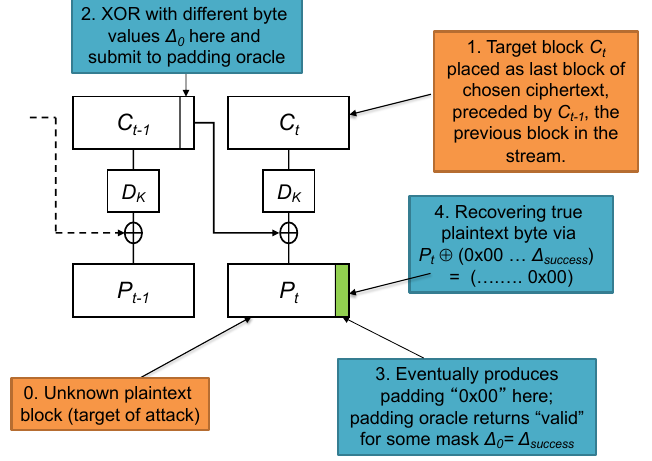
\includegraphics[scale=0.6]{images/cbc-padding-oracle-attack.png}
    \caption{Padding Oracle Attack on CBC mode}
    \label{fig:cbc-padding-oracle-attack}
\end{figure}

\paragraph{Predictable IVs}
Random IVs are not just theoretically relevant for IND-CPA security of CBC mode.
Consider the following steps (see \autoref{fig:cbc-predictable-iv}):
\begin{enumerate}
\item $\A$ queries LoR oracle with $(P_0, P_1)$
\item Oracle responds with $C = C_0||C_1$ where $C_1 = E_K(P_b \xor C_0)$
\item $\A$ predicts next $IV=C_0'$
\item $\A$ queries $P_0 \xor C_0 \xor C_0'$
\item $\implies b = 0 \iff P_b = P_0 \iff C_1 = C_1' \implies$ breaks IND-CPA security
\end{enumerate}

In practice: systems may use \emph{IV chaining} (use the last ciphertext as the next IV, in order to avoid having to sample new randomness).
E.g.: SSLv3, TLS 1.0, SSH in CBC mode.
See also the BEAST attack on TLS.

\begin{figure}[h]
    \centering
	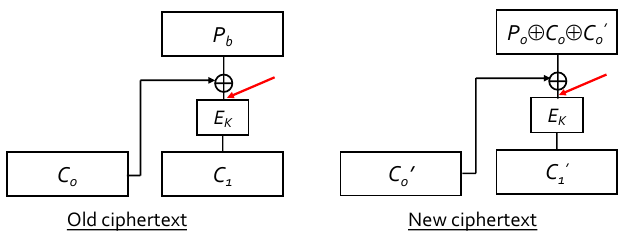
\includegraphics[scale=0.6]{images/cbc-predictable-iv.png}
    \caption{Attack on predictable IVs in CBC mode}
    \label{fig:cbc-predictable-iv}
\end{figure}



\subsection{Hash Functions}


\subsection{Message Authentication Codes MACs}


\subsection{Authenticated Encryption}

